% Options for packages loaded elsewhere
\PassOptionsToPackage{unicode}{hyperref}
\PassOptionsToPackage{hyphens}{url}
\PassOptionsToPackage{dvipsnames,svgnames,x11names}{xcolor}
%
\documentclass[fleqn,10pt]{wlscirep}

\usepackage{lineno}

\linenumbers


\usepackage{amsmath,amssymb}
\usepackage{iftex}
\ifPDFTeX
  \usepackage[T1]{fontenc}
  \usepackage[utf8]{inputenc}
  \usepackage{textcomp} % provide euro and other symbols
\else % if luatex or xetex
  \usepackage{unicode-math}
  \defaultfontfeatures{Scale=MatchLowercase}
  \defaultfontfeatures[\rmfamily]{Ligatures=TeX,Scale=1}
\fi
\usepackage{lmodern}
\ifPDFTeX\else  
    % xetex/luatex font selection
\fi
% Use upquote if available, for straight quotes in verbatim environments
\IfFileExists{upquote.sty}{\usepackage{upquote}}{}
\IfFileExists{microtype.sty}{% use microtype if available
  \usepackage[]{microtype}
  \UseMicrotypeSet[protrusion]{basicmath} % disable protrusion for tt fonts
}{}
\makeatletter
\@ifundefined{KOMAClassName}{% if non-KOMA class
  \IfFileExists{parskip.sty}{%
    \usepackage{parskip}
  }{% else
    \setlength{\parindent}{0pt}
    \setlength{\parskip}{6pt plus 2pt minus 1pt}}
}{% if KOMA class
  \KOMAoptions{parskip=half}}
\makeatother
\usepackage{xcolor}
\setlength{\emergencystretch}{3em} % prevent overfull lines
\setcounter{secnumdepth}{-\maxdimen} % remove section numbering
% Make \paragraph and \subparagraph free-standing
\ifx\paragraph\undefined\else
  \let\oldparagraph\paragraph
  \renewcommand{\paragraph}[1]{\oldparagraph{#1}\mbox{}}
\fi
\ifx\subparagraph\undefined\else
  \let\oldsubparagraph\subparagraph
  \renewcommand{\subparagraph}[1]{\oldsubparagraph{#1}\mbox{}}
\fi


\usepackage{color}
\usepackage{fancyvrb}
\newcommand{\VerbBar}{|}
\newcommand{\VERB}{\Verb[commandchars=\\\{\}]}
\DefineVerbatimEnvironment{Highlighting}{Verbatim}{commandchars=\\\{\}}
% Add ',fontsize=\small' for more characters per line
\usepackage{framed}
\definecolor{shadecolor}{RGB}{241,243,245}
\newenvironment{Shaded}{\begin{snugshade}}{\end{snugshade}}
\newcommand{\AlertTok}[1]{\textcolor[rgb]{0.68,0.00,0.00}{#1}}
\newcommand{\AnnotationTok}[1]{\textcolor[rgb]{0.37,0.37,0.37}{#1}}
\newcommand{\AttributeTok}[1]{\textcolor[rgb]{0.40,0.45,0.13}{#1}}
\newcommand{\BaseNTok}[1]{\textcolor[rgb]{0.68,0.00,0.00}{#1}}
\newcommand{\BuiltInTok}[1]{\textcolor[rgb]{0.00,0.23,0.31}{#1}}
\newcommand{\CharTok}[1]{\textcolor[rgb]{0.13,0.47,0.30}{#1}}
\newcommand{\CommentTok}[1]{\textcolor[rgb]{0.37,0.37,0.37}{#1}}
\newcommand{\CommentVarTok}[1]{\textcolor[rgb]{0.37,0.37,0.37}{\textit{#1}}}
\newcommand{\ConstantTok}[1]{\textcolor[rgb]{0.56,0.35,0.01}{#1}}
\newcommand{\ControlFlowTok}[1]{\textcolor[rgb]{0.00,0.23,0.31}{#1}}
\newcommand{\DataTypeTok}[1]{\textcolor[rgb]{0.68,0.00,0.00}{#1}}
\newcommand{\DecValTok}[1]{\textcolor[rgb]{0.68,0.00,0.00}{#1}}
\newcommand{\DocumentationTok}[1]{\textcolor[rgb]{0.37,0.37,0.37}{\textit{#1}}}
\newcommand{\ErrorTok}[1]{\textcolor[rgb]{0.68,0.00,0.00}{#1}}
\newcommand{\ExtensionTok}[1]{\textcolor[rgb]{0.00,0.23,0.31}{#1}}
\newcommand{\FloatTok}[1]{\textcolor[rgb]{0.68,0.00,0.00}{#1}}
\newcommand{\FunctionTok}[1]{\textcolor[rgb]{0.28,0.35,0.67}{#1}}
\newcommand{\ImportTok}[1]{\textcolor[rgb]{0.00,0.46,0.62}{#1}}
\newcommand{\InformationTok}[1]{\textcolor[rgb]{0.37,0.37,0.37}{#1}}
\newcommand{\KeywordTok}[1]{\textcolor[rgb]{0.00,0.23,0.31}{#1}}
\newcommand{\NormalTok}[1]{\textcolor[rgb]{0.00,0.23,0.31}{#1}}
\newcommand{\OperatorTok}[1]{\textcolor[rgb]{0.37,0.37,0.37}{#1}}
\newcommand{\OtherTok}[1]{\textcolor[rgb]{0.00,0.23,0.31}{#1}}
\newcommand{\PreprocessorTok}[1]{\textcolor[rgb]{0.68,0.00,0.00}{#1}}
\newcommand{\RegionMarkerTok}[1]{\textcolor[rgb]{0.00,0.23,0.31}{#1}}
\newcommand{\SpecialCharTok}[1]{\textcolor[rgb]{0.37,0.37,0.37}{#1}}
\newcommand{\SpecialStringTok}[1]{\textcolor[rgb]{0.13,0.47,0.30}{#1}}
\newcommand{\StringTok}[1]{\textcolor[rgb]{0.13,0.47,0.30}{#1}}
\newcommand{\VariableTok}[1]{\textcolor[rgb]{0.07,0.07,0.07}{#1}}
\newcommand{\VerbatimStringTok}[1]{\textcolor[rgb]{0.13,0.47,0.30}{#1}}
\newcommand{\WarningTok}[1]{\textcolor[rgb]{0.37,0.37,0.37}{\textit{#1}}}

\providecommand{\tightlist}{%
  \setlength{\itemsep}{0pt}\setlength{\parskip}{0pt}}
\usepackage{longtable,booktabs,array}
\usepackage{calc} % for calculating minipage widths
% Correct order of tables after \paragraph or \subparagraph
\usepackage{etoolbox}
\makeatletter
\patchcmd\longtable{\par}{\if@noskipsec\mbox{}\fi\par}{}{}
\makeatother
% Allow footnotes in longtable head/foot
\IfFileExists{footnotehyper.sty}{\usepackage{footnotehyper}}{\usepackage{footnote}}
\makesavenoteenv{longtable}

\usepackage{graphicx}
\makeatletter
\def\maxwidth{\ifdim\Gin@nat@width>\linewidth\linewidth\else\Gin@nat@width\fi}
\def\maxheight{\ifdim\Gin@nat@height>\textheight\textheight\else\Gin@nat@height\fi}
\makeatother
% Scale images if necessary, so that they will not overflow the page
% margins by default, and it is still possible to overwrite the defaults
% using explicit options in \includegraphics[width, height, ...]{}
\setkeys{Gin}{width=\maxwidth,height=\maxheight,keepaspectratio}
% Set default figure placement to htbp
\makeatletter
\def\fps@figure{htbp}
\makeatother



\usepackage{orcidlink}
\usepackage{lineno}
\definecolor{mypink}{RGB}{219, 48, 122}
\RequirePackage[numbers,super]{natbib}
\makeatletter
\makeatother
\makeatletter
\makeatother
\makeatletter
\@ifpackageloaded{caption}{}{\usepackage{caption}}
\AtBeginDocument{%
\ifdefined\contentsname
  \renewcommand*\contentsname{Table of contents}
\else
  \newcommand\contentsname{Table of contents}
\fi
\ifdefined\listfigurename
  \renewcommand*\listfigurename{List of Figures}
\else
  \newcommand\listfigurename{List of Figures}
\fi
\ifdefined\listtablename
  \renewcommand*\listtablename{List of Tables}
\else
  \newcommand\listtablename{List of Tables}
\fi
\ifdefined\figurename
  \renewcommand*\figurename{Figure}
\else
  \newcommand\figurename{Figure}
\fi
\ifdefined\tablename
  \renewcommand*\tablename{Table}
\else
  \newcommand\tablename{Table}
\fi
}
\@ifpackageloaded{float}{}{\usepackage{float}}
\floatstyle{ruled}
\@ifundefined{c@chapter}{\newfloat{codelisting}{h}{lop}}{\newfloat{codelisting}{h}{lop}[chapter]}
\floatname{codelisting}{Listing}
\newcommand*\listoflistings{\listof{codelisting}{List of Listings}}
\makeatother
\makeatletter
\@ifpackageloaded{caption}{}{\usepackage{caption}}
\@ifpackageloaded{subcaption}{}{\usepackage{subcaption}}
\makeatother
\makeatletter
\@ifpackageloaded{tcolorbox}{}{\usepackage[skins,breakable]{tcolorbox}}
\makeatother
\makeatletter
\@ifundefined{shadecolor}{\definecolor{shadecolor}{rgb}{.97, .97, .97}}
\makeatother
\makeatletter
\makeatother
\makeatletter
\makeatother
\ifLuaTeX
  \usepackage{selnolig}  % disable illegal ligatures
\fi
\IfFileExists{bookmark.sty}{\usepackage{bookmark}}{\usepackage{hyperref}}
\IfFileExists{xurl.sty}{\usepackage{xurl}}{} % add URL line breaks if available
\urlstyle{same} % disable monospaced font for URLs
\hypersetup{
  pdftitle={Data Descriptor Title (110 character maximum, inc. spaces)},
  pdfauthor={Christine Author; Derek Author; Sam Author},
  pdfkeywords={keyword 1, keyword 2, keyword 3, keyword 4},
  colorlinks=true,
  linkcolor={blue},
  filecolor={Maroon},
  citecolor={Blue},
  urlcolor={blue},
  pdfcreator={LaTeX via pandoc}}


\title{Data Descriptor Title (110 character maximum, inc. spaces)}

                                                                                    \author[1\dag]{Christine
Author}
                                                                                                                                                \author[1\dag]{Derek
Author}
                                                                                                                                                \author[2*]{Sam
Author\orcidlink{0000-0001-1122-3555}}
                                                                
    \affil[1]{Big Old University, University Road, City, Country}
    \affil[2]{Research Institute, Main Road, City, Country}

                    \affil[*]{corresponding author(s): Sam Author Sam
Author@researchinst.org}
    
\affil[$\dag$]{these authors contributed equally to this work}

\begin{abstract}
This is a manuscript template for Data Descriptor submissions to
\textbf{Scientific Data} \url{http://www.nature.com/scientificdata}. The
abstract must be no longer than 170 words, and should succinctly
describe the study, the assay(s) performed, the resulting data, and the
reuse potential, but should not make any claims regarding new scientific
findings. No references are allowed in this section.
\end{abstract}
\begin{document}
\flushbottom
\maketitle
%  Click the title above to edit the author information and abstract

\thispagestyle{empty}\ifdefined\Shaded\renewenvironment{Shaded}{\begin{tcolorbox}[enhanced, interior hidden, frame hidden, breakable, borderline west={3pt}{0pt}{shadecolor}, boxrule=0pt, sharp corners]}{\end{tcolorbox}}\fi

Please note: Abbreviations should be introduced at the first mention in
the main text -- no abbreviations lists or tables should be included.
Structure of the main text is provided below.

\hypertarget{background-summary}{%
\section{Background \& Summary}\label{background-summary}}

(700 words maximum) An overview of the study design, the assay(s)
performed, and the created data, including any background information
needed to put this study in the context of previous work and the
literature. The section should also briefly outline the broader goals
that motivated the creation of this dataset and the potential reuse
value. We also encourage authors to include a figure that provides a
schematic overview of the study and assay(s) design. The Background \&
Summary should not include subheadings. This section and the other main
body sections of the manuscript should include citations to the
literature as needed.

\hypertarget{methods}{%
\section{Methods}\label{methods}}

The Methods should include detailed text describing any steps or
procedures used in producing the data, including full descriptions of
the experimental design, data acquisition assays, and any computational
processing (e.g.~normalization, image feature extraction). See the
detailed section in our submission guidelines for advice on writing a
transparent and reproducible methods section. Related methods should be
grouped under corresponding subheadings where possible, and methods
should be described in enough detail to allow other researchers to
interpret and repeat, if required, the full study. Specific data outputs
should be explicitly referenced via data citation (see Data Records and
Citing Data, below).

Authors should cite previous descriptions of the methods under use, but
ideally the method descriptions should be complete enough for others to
understand and reproduce the methods and processing steps without
referring to associated publications. There is no limit to the length of
the Methods section. Subheadings should not be numbered.

\hypertarget{subsection}{%
\subsection{Subsection}\label{subsection}}

Example text under a subsection. Bulleted lists may be used where
appropriate, e.g.

\begin{itemize}
\tightlist
\item
  First item
\item
  Second item
\end{itemize}

\hypertarget{third-level-subsection}{%
\subsubsection{Third-level subsection}\label{third-level-subsection}}

Topical subheadings are allowed.

\hypertarget{data-records}{%
\section{Data Records}\label{data-records}}

The Data Records section should be used to explain each data record
associated with this work, including the repository where this
information is stored, and to provide an overview of the data files and
their formats. Each external data record should be cited numerically in
the text of this section, for example \citep{Hao:gidmaps:2014}, and
included in the main reference list as described below. A data citation
should also be placed in the subsection of the Methods containing the
data-collection or analytical procedure(s) used to derive the
corresponding record. Providing a direct link to the dataset may also be
helpful to readers \url{https://doi.org/10.6084/m9.figshare.853801}.

Tables should be used to support the data records, and should clearly
indicate the samples and subjects (study inputs), their provenance, and
the experimental manipulations performed on each (please see `Tables'
below). They should also specify the data output resulting from each
data-collection or analytical step, should these form part of the
archived record.

\hypertarget{technical-validation}{%
\section{Technical Validation}\label{technical-validation}}

This section presents any experiments or analyses that are needed to
support the technical quality of the dataset. This section may be
supported by figures and tables, as needed. This is a required section;
authors must present information justifying the reliability of their
data.

\hypertarget{usage-notes}{%
\section{Usage Notes}\label{usage-notes}}

The Usage Notes should contain brief instructions to assist other
researchers with reuse of the data. This may include discussion of
software packages that are suitable for analysing the assay data files,
suggested downstream processing steps (e.g.~normalization, etc.), or
tips for integrating or comparing the data records with other datasets.
Authors are encouraged to provide code, programs or data-processing
workflows if they may help others understand or use the data. Please see
our code availability policy for advice on supplying custom code
alongside Data Descriptor manuscripts.

For studies involving privacy or safety controls on public access to the
data, this section should describe in detail these controls, including
how authors can apply to access the data, what criteria will be used to
determine who may access the data, and any limitations on data use.

\hypertarget{code-availability}{%
\section{Code availability}\label{code-availability}}

For all studies using custom code in the generation or processing of
datasets, a statement must be included under the heading ``Code
availability'', indicating whether and how the code can be accessed,
including any restrictions to access. This section should also include
information on the versions of any software used, if relevant, and any
specific variables or parameters used to generate, test, or process the
current dataset.

\hypertarget{references}{%
\section{References}\label{references}}

\renewcommand{\bibsection}{}
\bibliography{bibliography.bib}

\hypertarget{acknowledgements-not-compulsory}{%
\section{Acknowledgements (not
compulsory)}\label{acknowledgements-not-compulsory}}

Acknowledgements should be brief, and should not include thanks to
anonymous referees and editors, or effusive comments. Grant or
contribution numbers may be acknowledged.

\hypertarget{author-contributions-statement}{%
\section{Author contributions
statement}\label{author-contributions-statement}}

Must include all authors, identified by initials, for example: A.A.
conceived the experiment(s), A.A. and B.A. conducted the experiment(s),
C.A. and D.A. analysed the results. All authors reviewed the manuscript.

\hypertarget{competing-interests-mandatory-statement}{%
\section{Competing interests (mandatory
statement)}\label{competing-interests-mandatory-statement}}

The corresponding author is responsible for providing a
\href{https://www.nature.com/sdata/policies/editorial-and-publishing-policies\#competing}{competing
interest statement} on behalf of all authors of the paper. This
statement must be included in the submitted article file.

\hypertarget{figures-tables}{%
\section{Figures \& Tables}\label{figures-tables}}

Figures, tables, and their legends, should be included at the end of the
document. Figures and tables can be referenced in Quarto using
\texttt{!{[}caption{]}(source\_to\_figure.jpg)}, e.g.
Figure~\ref{fig-stream} and Table~\ref{tbl-example}.

\begin{figure}

{\centering 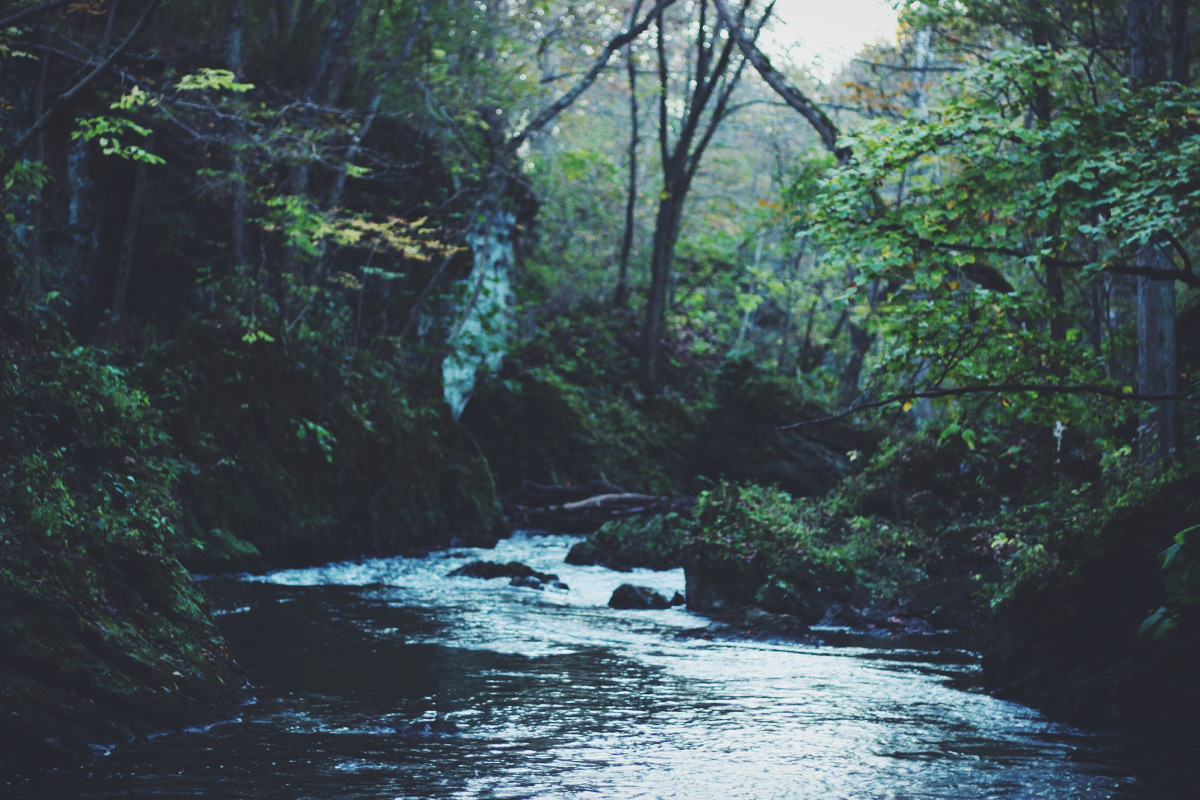
\includegraphics{stream.jpg}

}

\caption{\label{fig-stream}Legend (350 words max). Example legend text.}

\end{figure}

\hypertarget{tbl-example}{}
\begin{longtable}[]{@{}lll@{}}
\caption{\label{tbl-example}Legend (350 words max). Example legend
text.}\tabularnewline
\toprule\noalign{}
Condition & n & p \\
\midrule\noalign{}
\endfirsthead
\toprule\noalign{}
Condition & n & p \\
\midrule\noalign{}
\endhead
\bottomrule\noalign{}
\endlastfoot
A & 5 & 0.1 \\
B & 10 & 0.01 \\
\end{longtable}

Authors are encouraged to provide one or more tables that provide basic
information on the main `inputs' to the study (e.g.~samples,
participants, or information sources) and the main data outputs of the
study. Tables in the manuscript should generally not be used to present
primary data (i.e.~measurements). Tables containing primary data should
be submitted to an appropriate data repository.

Tables may be provided within the {\LaTeX} document or as separate files
(tab-delimited text or Excel files). Legends, where needed, should be
included here. Generally, a Data Descriptor should have fewer than ten
Tables, but more may be allowed when needed. Tables may be of any size,
but only Tables which fit onto a single printed page will be included in
the PDF version of the article (up to a maximum of three).

Due to typesetting constraints, tables that do not fit onto a single A4
page cannot be included in the PDF version of the article and will be
made available in the online version only. Any such tables must be
labelled in the text as `Online-only' tables and numbered separately
from the main table list e.g.~`Table 1, Table 2, Online-only Table 1'
etc.

Everything for the extensions is in \texttt{\_extensions}. See Quarto
doc for details.

\begin{itemize}
\item
  In \texttt{partials}, you'll find the \texttt{.tex} partials that can
  be used and should be removed or tweaked,s
\item
  Your extension can make shortcodes and lua filters available. This
  document shows the effect of the one provided in the \texttt{aft}
  format.
\item
  \texttt{aft} format sets some defaults which are different from
  \texttt{pdf} or \texttt{html}, link setting links to URL in read
  inside PDF output.
\end{itemize}

Source repository for this template format can found on
\href{https://github.com/quarto-journals/article-format-template}{Github}

\hypertarget{technical-validation-1}{%
\section{Technical Validation}\label{technical-validation-1}}

In this folder you'll find everything that defines the extensions which
could be installed using \texttt{quarto\ install\ extension} or be part
of the template when using \texttt{quarto\ use\ template}

\hypertarget{format-metadata}{%
\subsection{Format Metadata}\label{format-metadata}}

\textasciitilde{} This is in \texttt{\_extension.yml} is where all the
metadata about the format are defined so that Quarto knows what to use.
Adapt this file for you own template.

\hypertarget{partials}{%
\subsection{Partials}\label{partials}}

\textasciitilde{} In \texttt{partials}, there are the \texttt{.tex}
files that will be used as Pandoc's template. We provide here all the
partials supported by Quarto and custom one for this format. Quarto
allows to provide partials to ease the process of tweaking the default
latex Pandoc's template and keeping it up to date.\\
This template repo contains all the relevant partials that you can use
with Quarto \emph{as example}. We only tweaked \texttt{title.tex} to
show the usage of a custom partials called \texttt{\_custom.tex}.\\
\textbf{Only keep the partials that you need to tweak for the format you
are creating}

\begin{verbatim}
If you need to completely change the default template (i.g customizing partials is not enough), then you need to provide your own template to Pandoc based on [`template.tex`](https://github.com/quarto-dev/quarto-cli/blob/main/src/resources/formats/pdf/pandoc/template.tex) and also using partials or not. This can be provided using the `template` YAML key in `_extension.yml` for Quarto to use it. 

This is considered advanced configuration as it will be harder to maintain than only using partials but could be required for some specific format. Be aware that this may lead to loose some Pandoc or Quarto features tied to default `template.tex` content if you remove some specific parts.
\end{verbatim}

\hypertarget{usage-notes-1}{%
\section{Usage Notes}\label{usage-notes-1}}

\textasciitilde{} Most of the time, custom formats will need Lua filters
to provide specific features like cross format supports or provides
custom shortcodes through the Quarto extension mechanism. Those filters
will be available to the user and could be used in the custom formats
(according to \texttt{\_extensions} metadata). We have provided two
examples:

\begin{verbatim}
- `color-text.lua`, a Lua filter used to add color to inline text for PDF and HTML outputs using the same Markdown syntax
- `shorcodes.lua`, a Lua filter which follow [Quarto custom shortcodes](https://quarto.org/docs/authoring/shortcodes.html#custom-shortcodes) guidelines to provide a `` shortcode to nicely print LaTeX in PDF and HTML. 

**Remove or replace with your own Lua filters**
\end{verbatim}

\hypertarget{code-availability-1}{%
\section{Code availability}\label{code-availability-1}}

\textasciitilde{} Resources required by the format needs to be
available. We have provided two examples:

\begin{verbatim}
- `te.bst` is a biblio style file for demo. It has been downloaded from https://www.economics.utoronto.ca/osborne/latex/TEBST.HTM (http://econtheory.org/technical/te.bst) - Licence [LPPL](https://www.latex-project.org/lppl/)
- `aft.cls` is a dummy class file for this example format. It is a copy of official `article.cls`, the one provided in LaTeX installation (i.e at `kpsewhich article.cls`) and renamed as example (Licence LaTeX Project Public License)
- `custom.scss` is a style file to have a custom theme for our HTML format so that our Lua filter feature `color-tex.lua` works.

Those files are referenced within the `_extension.yml` to be used with our example format.

**Remove and replace with your own resources**
\end{verbatim}

\begin{description}
\item[\texttt{.quartoignore}]
Sometimes it is useful to have some files only needed for reference or
for development. They should be available in the source repository but
not downloaded to the user when \texttt{quarto\ use\ template} is used.

\textbf{Use \texttt{.quartoignore} to register such file and folder (one
file or folder per line)}
\item[\texttt{style-guide} folder]
For \texttt{quarto-journals} format, use \texttt{style-guide} folder to
include any documentation and resourced used for format creation, like a
journal style guide or original \texttt{.tex} template. This folder is
already added in \texttt{.quartoignore} in this example repo.

\textbf{Remove, rename or add to this folder}
\item[\texttt{template.qmd}]
This file is the template document that shows how to use the custom
format. It will be downloaded with other resource by
\texttt{quarto\ use\ template}, and even offered to be renamed if the
name \texttt{template.qmd} is used.

This file will usually use the custom format (here \texttt{aft-pdf} and
\texttt{aft-html}) and show how to use the template. When you'll copy
this template, you should be able to render this document to the demo
format.

\textbf{Adapt this file to provide a suitable template for your custom
format}
\item[Other files]
Other files are needed by the template and are usually user provided -
they are not part of the custom format.

Here \texttt{bibliography.bib} is here to demo the usage of the bst file
from the custom format.

\textbf{Remove this file and provide a suitable one for your template}
\end{description}

\newpage{}

\hypertarget{checklist-creating-a-custom-format}{%
\subsection{Checklist: Creating a custom
format}\label{checklist-creating-a-custom-format}}

Here is the checklist to help you know what to modify:

\begin{itemize}
\tightlist
\item
  Read the resources mentioned at the top,
\item
  Use this template repo to create a new repository for your format
  (Click on ``Use this template'' to create new github repo)
\item
  Once you are acquainted with the content, remove the resources that
  are there only as example (see above)
\item
  Update README by replacing \texttt{aft} and
  \texttt{Article\ Format\ Template} mentions for your journal format
\item
  Keep only the template partials that you need to tweak, and add custom
  ones if needed
\item
  Add any Lua filters for shortcodes and other that would be useful to
  create the expected output format
\item
  Add any external resource your format will need, and that should be
  part of the extension format that will be downloaded,
\item
  Check \texttt{\_extension.yml} is updated correctly
\item
  Modify the skeleton \texttt{template.qmd} to your format and add any
  required resources to be downloaded to user.
\item
  Check \texttt{.quartoignore} is updated which everything that should
  not be downloaded.
\item
  Publish a demo of you format to github pages of the repo by using
  \texttt{quarto\ publish} command
\end{itemize}

\hypertarget{demo-of-some-features-found-in-this-demo-journal-template}{%
\subsection{Demo of some features found in this demo journal
template}\label{demo-of-some-features-found-in-this-demo-journal-template}}

\hypertarget{sec-shortcode}{%
\subsubsection{Shortcode demo}\label{sec-shortcode}}

PDF are rendered using {\LaTeX} but it is best if one can use a Markdown
syntax for cross format support.

\texttt{} used in source is a shortcode syntax where the shortcode is
included in the extension folder \texttt{\_extensions}

\hypertarget{sec-chunks}{%
\subsubsection{Code chunk}\label{sec-chunks}}

This format hide chunks by default as option has been set in
\texttt{\_extension.yml} file.

But you can set \texttt{echo} option to \texttt{true} locally in the
chunk

\begin{Shaded}
\begin{Highlighting}[]
\NormalTok{m\_pois }\OtherTok{\textless{}{-}} \FunctionTok{glm}\NormalTok{(Days }\SpecialCharTok{\textasciitilde{}}\NormalTok{ (Eth }\SpecialCharTok{+}\NormalTok{ Sex }\SpecialCharTok{+}\NormalTok{ Age }\SpecialCharTok{+}\NormalTok{ Lrn)}\SpecialCharTok{\^{}}\DecValTok{2}\NormalTok{, }\AttributeTok{data =}\NormalTok{ quine, }\AttributeTok{family =}\NormalTok{ poisson)}
\FunctionTok{summary}\NormalTok{(m\_pois)}
\end{Highlighting}
\end{Shaded}

\begin{verbatim}

Call:
glm(formula = Days ~ (Eth + Sex + Age + Lrn)^2, family = poisson, 
    data = quine)

Coefficients: (1 not defined because of singularities)
            Estimate Std. Error z value Pr(>|z|)    
(Intercept)  2.93246    0.09826  29.843  < 2e-16 ***
EthN        -0.17399    0.12134  -1.434   0.1516    
SexM        -0.71452    0.12229  -5.843 5.14e-09 ***
AgeF1       -0.04270    0.12691  -0.336   0.7365    
AgeF2       -0.08632    0.16164  -0.534   0.5933    
AgeF3       -0.15290    0.11898  -1.285   0.1987    
LrnSL        0.21608    0.14558   1.484   0.1377    
EthN:SexM    0.43902    0.09208   4.768 1.86e-06 ***
EthN:AgeF1  -0.92889    0.14657  -6.337 2.34e-10 ***
EthN:AgeF2  -1.33398    0.13504  -9.879  < 2e-16 ***
EthN:AgeF3  -0.11242    0.13478  -0.834   0.4042    
EthN:LrnSL   0.26415    0.11378   2.322   0.0203 *  
SexM:AgeF1  -0.05565    0.16303  -0.341   0.7328    
SexM:AgeF2   1.09942    0.15281   7.195 6.26e-13 ***
SexM:AgeF3   1.15949    0.13859   8.366  < 2e-16 ***
SexM:LrnSL   0.04143    0.13718   0.302   0.7627    
AgeF1:LrnSL -0.13019    0.15688  -0.830   0.4066    
AgeF2:LrnSL  0.37340    0.14563   2.564   0.0103 *  
AgeF3:LrnSL       NA         NA      NA       NA    
---
Signif. codes:  0 '***' 0.001 '**' 0.01 '*' 0.05 '.' 0.1 ' ' 1

(Dispersion parameter for poisson family taken to be 1)

    Null deviance: 2073.5  on 145  degrees of freedom
Residual deviance: 1368.7  on 128  degrees of freedom
AIC: 1993.1

Number of Fisher Scoring iterations: 5
\end{verbatim}

\hypertarget{sec-summary}{%
\subsubsection{Text color}\label{sec-summary}}

Our format makes applying color on inline text possible using the
\texttt{{[}content{]}\{color=\textless{}name\textgreater{}\}} syntax.
Let's see an example.

Here we are using a special feature of our format which is the coloring
because \textcolor{mypink}{pink is a \textbf{nice} color}.

This is possible thanks to the Lua Filter included in the custom
extension format.

\hypertarget{using-references}{%
\subsubsection*{Using references}\label{using-references}}
\addcontentsline{toc}{subsubsection}{Using references}

I did not read this book \citep{behringer2014manipulating} but it must
be interesting.

Differences between \texttt{aft-html} and \texttt{aft-pdf}:

\begin{itemize}
\tightlist
\item
  For the HTML format, we are using Pandoc citeproc to include the
  bibliography. Here \texttt{reference-section-title} controls the title
  for the chapter that will be used.
\item
  For the PDF format, \texttt{natbib} is used by default and the
  bibliography is included with a title by the LaTeX template.
\end{itemize}




\end{document}
